% Created 2020-04-30 jue 16:59
% Intended LaTeX compiler: pdflatex
\documentclass[xcolor={usenames,svgnames,dvipsnames}]{beamer}
\usepackage[utf8]{inputenc}
\usepackage[T1]{fontenc}
\usepackage{graphicx}
\usepackage{grffile}
\usepackage{longtable}
\usepackage{wrapfig}
\usepackage{rotating}
\usepackage[normalem]{ulem}
\usepackage{amsmath}
\usepackage{textcomp}
\usepackage{amssymb}
\usepackage{capt-of}
\usepackage{hyperref}
\usepackage{color}
\usepackage{listings}
\usepackage{mathpazo}
\usepackage{gensymb}
\usepackage{amsmath}
\usepackage{esdiff}
\usepackage{steinmetz}
\bibliographystyle{plain}
\AtBeginSubsection[]{\begin{frame}[plain]\tableofcontents[currentsubsection,sectionstyle=show/shaded,subsectionstyle=show/shaded/hide]\end{frame}}
\AtBeginSection[]{\begin{frame}[plain]\tableofcontents[currentsection,hideallsubsections]\end{frame}}
\usepackage[emulate=units]{siunitx}
\sisetup{fraction=nice, decimalsymbol=comma, retain-unity-mantissa = false}
\newunit{\wattpeak}{Wp}
\newunit{\watthour}{Wh}
\newunit{\amperehour}{Ah}
\hypersetup{colorlinks=true, linkcolor=Blue, urlcolor=Blue}
\renewcommand{\thefootnote}{\fnsymbol{footnote}}
\beamertemplatenavigationsymbolsempty
\setbeamertemplate{footline}[frame number]
\newcommand{\laplace}[1]{\mathbf{#1}(\mathbf{s})}
\newcommand{\slp}{\mathbf{s}}
\newcommand{\fasor}[1]{\mathbf{#1}(\omega)}
\newcommand{\atan}{\mathrm{atan}}
\setbeamercolor{alerted text}{fg=blue!50!black} \setbeamerfont{alerted text}{series=\bfseries}
\usetheme[hideothersubsections]{Goettingen}
\usecolortheme{rose}
\usefonttheme{serif}
\author{Oscar Perpiñán Lamigueiro}
\date{Septiembre 2018}
\title{Introducción al Régimen Transitorio}
\subtitle{Teoría de Circuitos III}
\hypersetup{
 pdfauthor={Oscar Perpiñán Lamigueiro},
 pdftitle={Introducción al Régimen Transitorio},
 pdfkeywords={},
 pdfsubject={},
 pdfcreator={Emacs 26.1 (Org mode 9.3.6)}, 
 pdflang={Spanish}}
\begin{document}

\maketitle

\section{¿Qué es el régimen transitorio?}
\label{sec:orgeab92ea}
\begin{frame}[label={sec:org8fae7e5}]{Permanente y Estacionario}
\begin{block}{Régimen permanente o estacionario}
Las tensiones y corrientes de un circuito son constantes (continua) o periódicas (alterna) (circuito estabilizado)
\end{block}
\begin{block}{Régimen transitorio}
\begin{itemize}
\item Para alcanzar el régimen permanente (o para alternar entre dos regímenes permanentes) el circuito atraviesa el régimen transitorio.
\item Posibles cambios: activación o apagado de fuentes, cambio en las cargas, cambio en el circuito (línea).
\item En general, el estado transitorio es indeseado en sistemas eléctricos, pero provocado en sistemas electrónicos.
\end{itemize}
\end{block}
\end{frame}

\begin{frame}[label={sec:orgb7fd69d}]{Acumulación de Energía}
\begin{block}{Régimen Permanente}
\alert{Energía acumulada} en \alert{bobinas} y \alert{condensadores}
\end{block}
\begin{block}{Régimen Estacionario}
\begin{itemize}
\item \alert{Redistribución} y \alert{disipación} de energía acumulada.
\item La redistribución de energía \alert{no} se puede realizar de forma \alert{inmediata}
\item \alert{Duración corta} (\(\si{\micro\second}\)) pero superior a 0, dependiendo de \alert{relación entre acumulación y disipación} (resistencia).
\end{itemize}
\end{block}
\end{frame}

\section{Métodos de resolución}
\label{sec:orgea131ae}

\begin{frame}[label={sec:org51ccf0a}]{Análisis Clásico}
\begin{itemize}
\item Formulación de las ecuaciones integro-diferenciales y resolución \alert{directa}.
\end{itemize}
\[
LC \diff[2]{u_c}{t} + RC \diff{u_c}{t} + u_c = 0
\]
\begin{itemize}
\item Las \alert{condiciones iniciales} determinan las constantes de integración.
\item Fácil de aplicar a \alert{circuitos simples} (primer y segundo orden, uno o dos elementos de acumulación).
\item No es apropiado para circuitos de orden superior a 2.
\item Permite comprensión del funcionamiento del circuito.
\end{itemize}
\end{frame}
\begin{frame}[label={sec:orga8b652c}]{Transformada de Laplace}
\begin{itemize}
\item Transforma las ecuaciones integro-diferenciales en ecuaciones algebraicas de una variable compleja.
\end{itemize}
\[
LC s^2 + RC s + 1 = 0  
\]
\begin{itemize}
\item Incorpora las condiciones iniciales directamente en las ecuaciones algebraicas.
\item Método sistemático y potente, adecuado para cualquier tipo de circuito.
\end{itemize}
\end{frame}
\begin{frame}[label={sec:org67b92a8}]{Variables de estado}
\begin{itemize}
\item Método proveniente de la ingeniería de control.
\item Las variables de estado son aquellas que definen la evolución de un sistema.
\begin{itemize}
\item En circuitos eléctricos: tensión de condensadores, corriente de bobinas.
\end{itemize}
\item El sistema evoluciona a través de diferentes estados según los cambios en la energía acumulada: \alert{trayectoria del sistema}.
\item Representa el sistema mediante una \alert{ecuación diferencial matricial}:
\end{itemize}
\[
  \diff{\mathbf{x}}{t} = f\{\mathbf{x}, \mathbf{u}, t\}
  \]
\begin{itemize}
\item Método sistemático y potente, adecuado para resolución con ordenador.
\end{itemize}
\end{frame}
\section{Condiciones iniciales}
\label{sec:org099a045}
\begin{frame}[label={sec:orgf6de9cd}]{Respuesta completa de una red lineal}
\begin{itemize}
\item La respuesta completa de una red lineal a un cambio tiene dos componentes:
\begin{itemize}
\item Respuesta \alert{natural} o propia (sin fuentes, determinada únicamente por la configuración del circuito)
\item Respuesta \alert{forzada} o particular (determinada por las fuentes existentes, \(t = \infty\)).
\end{itemize}
\end{itemize}
\[
 f(t) = f_n(t) + f_\infty(t) 
 \]
\begin{itemize}
\item Las constantes de integración de la respuesta natural se determinan con las condiciones iniciales del circuito.
\end{itemize}
\end{frame}

\begin{frame}[label={sec:org1019cbe}]{Condiciones iniciales}
\begin{itemize}
\item \alert{Condiciones Iniciales}: estado del circuito en el instante temporal en el que se produce el cambio (p.ej. apertura de interruptor).
\item Este instante temporal se representa habitualmente con \(t = 0\).
\end{itemize}
\end{frame}
\begin{frame}[label={sec:orgfcee067}]{\(t = 0^+\) y \(t = 0^-\)}
\begin{itemize}
\item El estado previo a la conmutación es \(t = 0^-\) 
\begin{itemize}
\item La topología del circuito es la anterior al cambio.
\end{itemize}
\item El estado posterior a la conmutación es \(t = 0^+\).
\begin{itemize}
\item La topología del circuito es la posterior al cambio.
\end{itemize}
\end{itemize}
\end{frame}
\begin{frame}[label={sec:org9438a2c}]{Resistencia}
\[
u(t) = R i(t)
\]

\begin{itemize}
\item No acumula energía: sigue los cambios de forma instantánea.
\end{itemize}
\end{frame}

\begin{frame}[label={sec:orgb1b746b}]{Inductancia}
\[
u(t) = L \diff{i_L(t)}{t}
\]

\[
i_L(t) = \frac{1}{L} \int^t_{-\infty}u(t) \mathrm{d}t
\]

\begin{itemize}
\item La corriente en una bobina no puede variar de forma abrupta (implica tensión infinita).
\end{itemize}
\[
i_L(0^-) = i_L(0^+)
\]
\end{frame}

\begin{frame}[label={sec:org667007a}]{Capacidad}
\[
i(t) = C \diff{u_C(t)}{t}
\]

\[
u(t) = \frac{1}{C} \int^t_{-\infty}i(t) \mathrm{d}t
\]

\begin{itemize}
\item La tensión en un condensador no puede variar de forma abrupta (implica corriente infinita).
\end{itemize}
\[
u_C(0^-) = u_C(0^+)
\]
\end{frame}
\begin{frame}[label={sec:orgc10d556}]{Circuitos Equivalentes}
\begin{itemize}
\item Sustituir fuentes de tensión \(u_g(t)\) por \(u_g(0^+)\).
\item Sustituir fuentes de corriente \(i_g(t)\) por \(i_g(0^+)\).
\item Sustituir bobinas por fuentes de corriente \(i_L(0^+)\).
\item Sustituir condensadores por fuentes de tensión \(u_C(0^+)\).
\item Calcular tensiones y corrientes en circuito.
\end{itemize}
\begin{center}
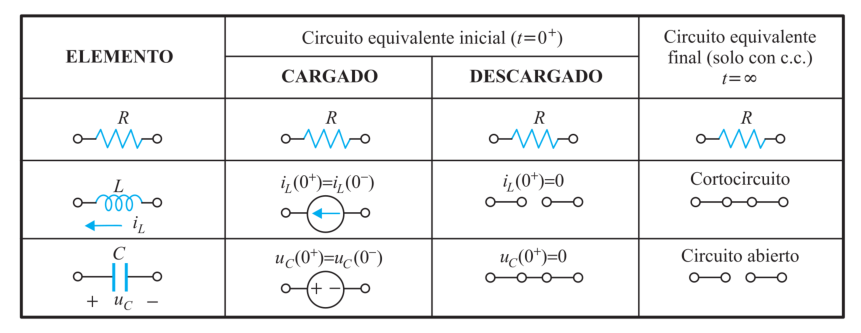
\includegraphics[width=.9\linewidth]{figs/CondicionesIniciales_CircuitosEquivalentes.pdf}
\end{center}
\end{frame}

\begin{frame}[label={sec:org1755650}]{Ejemplo}
\begin{block}{(Sep 2010) El interruptor lleva en la posición (1) desde un tiempo infinito, pasa a la posición (2)}
\begin{center}
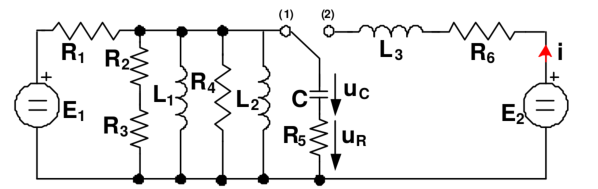
\includegraphics[width=.9\linewidth]{figs/ejemplo_condiciones_iniciales.pdf}
\end{center}
\end{block}
\end{frame}

\section{Funciones importantes}
\label{sec:orgda71b82}
\begin{frame}[label={sec:orgcbc688f}]{Función Escalón}
\[   
u(t - t_0) = 
     \begin{cases}
       0 &\quad t < t_0\\
       1 &\quad t > t_0\\
     \end{cases}
\]
\begin{center}
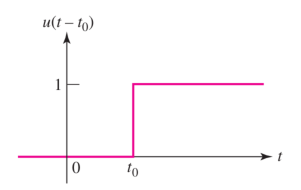
\includegraphics[width=.9\linewidth]{figs/funcion_escalon.pdf}
\end{center}
\end{frame}

\begin{frame}[label={sec:org14585dc}]{Función Escalón (\(t_0 = 0\))}
\[   
u(t) = 
     \begin{cases}
       0 &\quad t < 0\\
       1 &\quad t > 0\\
     \end{cases}
\]

\begin{center}
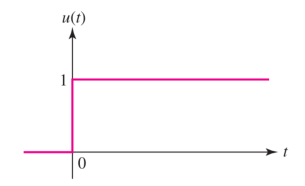
\includegraphics[width=.9\linewidth]{figs/funcion_escalon0.pdf}
\end{center}
\end{frame}

\begin{frame}[label={sec:org17e1c22}]{Función Exponencial}
\begin{itemize}
\item Es igual a su derivada.
\end{itemize}
\[
\diff{e^x}{x} = e^x
\]

\begin{itemize}
\item Es la solución habitual de las ecuaciones diferenciales.
\end{itemize}

\[
  \diff{f(t)}{t} = b f(t) \Rightarrow f(t) = A e^{bt}
\]
\end{frame}
\begin{frame}[label={sec:org9ac680c}]{Función Exponencial}
\begin{itemize}
\item Cuando el exponente es positivo la respuesta crece indefinidamente (circuito inestable).
\item Cuando el exponente es negativo la respuesta decae hasta 0 (circuito estable).
\end{itemize}
\begin{center}
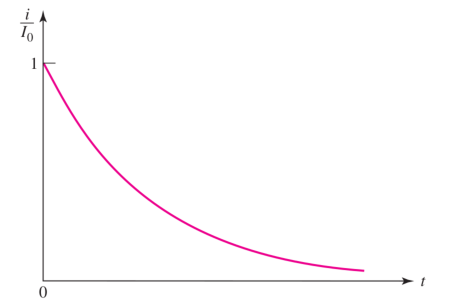
\includegraphics[width=.9\linewidth]{figs/exp_decreciente.pdf}
\end{center}
\end{frame}
\end{document}